% langLearnVar 
% Annual Cognitive Science Conference 2016

\documentclass[10pt,letterpaper]{article}

\usepackage{cogsci}
\usepackage{pslatex}
\usepackage{apacite2}
\usepackage{graphicx}
\usepackage{array,multirow}
 \usepackage{booktabs}
 \usepackage[table,xcdraw]{xcolor}



\newcommand*\rot{\rotatebox{90}}
\newcommand{\squeezeup}{\vspace{-1.5mm}}

\title{Linguistic pressures across multiple timescales}
\author{{\large \bf Molly Lewis} \\ \texttt{mll@stanford.edu}\\ Department of Psychology \\ Stanford University \\ 
\And {\large \bf Michael C. Frank} \\ \texttt{mcfrank@stanford.edu} \\ Department of Psychology \\ Stanford University \\ }

\begin{document}

\maketitle

\begin{abstract}

What accounts for the vast diversity in the world's languages? We explore one possibility: languages adapt to their linguistic environment ({\it Linguistic Niche Hypothesis}; Lupyan \& Dale, 2010). Recent studies have found support for this hypothesis through correlations between aspects of the environment and linguistic structure. We synthesize this previous work and find that languages spoken in cold, small regions to be more complex across a range of linguistic measures. We also test a novel prediction of the Linguistic Niche Hypothesis by examining the learnability of languages for L1 speakers. We find a trade-off between learnability for L1 and L2 speakers.

\textbf{Keywords:} 
Linguistic Niche Hypothesis; language evolution
\end{abstract}


%%%%% INTRODUCTION %%%%%%
\section{Introduction}
Why does language vary? Psychologists have made significant progress understanding linguistic variability in the domains of communicative interaction and children's developmental trajectories. In both cases, accounts rely on positing two pressures on the cognitive system---one internal and one external. In the case of communication, theorists argue that speakers are influenced by cognitive constraints (minimize effort) and by the needs of the communicative partner \cite<be understandable;>{horn1984}. In the case of acquisition, there are internal maturational constraints [CITE], as well as external pressures from the quality and quantity of linguistic input \cite{hart1995meaningful}. In the present paper, we explore the possibility that the same two pressures---system internal and external---may also account for variability in {\it language systems}. 

Central to this hypothesis is the notion of a timescale: there are different units of time over which processes operate, and processes at shorter timescales influence those at longer timescales \cite[Fig.\ 1]{blythe2015hierarchy}. At the shortest timescale  are  individual utterances in communicative interactions (pragmatics). At a longer timescale is language acquisition.  Both experimental and modeling work suggest that communicative interactions at the pragmatic timescale influence processes like word learning at the acquisition timescale \cite<e.g.,>{baldwin1991infants,mcmurray2012,frank2009a,frank2014inferring}.
%Critically, at both of these timescales, both internal and external pressures are thought to influence language (Fig. 1). 
\begin{figure}[b!]
\begin{center}
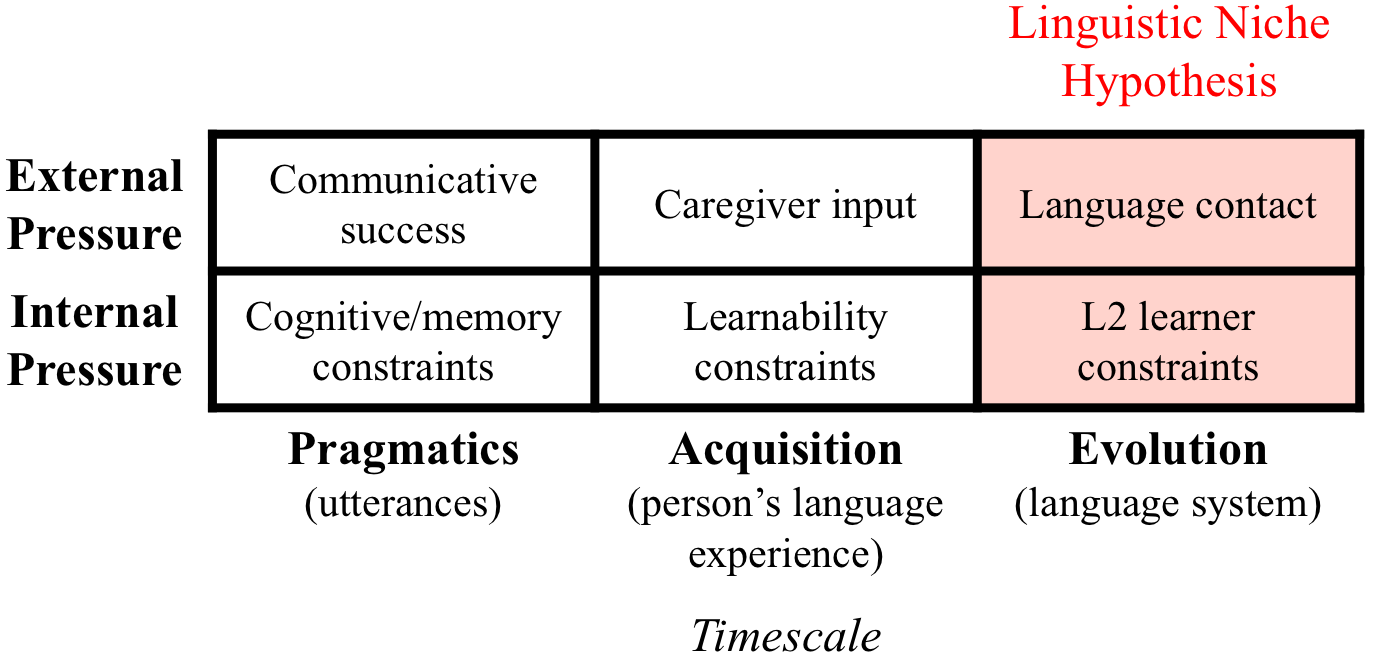
\includegraphics[scale = .35]{figs/timescales_table.png}
\end{center}
\vspace{-.5em}
\caption{Pressures on language internal and external to the cognitive system, at three different timescales. Brackets show examples of phenomena that result from a particular pressure at a particular timescale. The Linguistic Niche Hypothesis suggests that language evolution is influenced by the internal and external pressures in the particular environmental context in which a language is spoken.}
\label{fig:timescales}
\vspace{-1em}
\end{figure}


A third relevant timescale is language evolution: the timescale over which entire language systems change.   As for acquisition, there is evidence that language systems may be the product of processes at the pragmatic timescale. For example, languages universally structure semantic space to reflect optimal equilibria between communicative pressures  \cite<e.g.,>{kemp2012kinship,regier2007color,baddeley2009}.

%language evolution timescale, the goal is to explain variability at the level of language systems (Modern English vs.\ Old English; English vs.\ Thai).

However, the presence of communicative pressures at the pragmatic timescale is unable to explain cross-linguistic variability in linguistic structure. That is, why does Polish have rich morphology but English relatively sparse? A growing body of work argues that this variability may be due to cognitive constraints internal to the language learner \cite{chater2010language} as well as properties of the environmental context \cite{nettle2012social}. This hypothesis, termed the  {\it Linguistic Niche Hypothesis} \cite{lupyan2010language,wray2007consequences}, suggests that language systems adapt to the internal and external pressures of  the linguistic environment. %These pressures may come from external pressures, such as contact with other languages, as well as constraints by learners themselves. 

%from a range of sources, including the climate, the length of the growing season, or the demographic characteristics of the people who learn and speak the language. 


%An important aspect of this hypothesis is the timescale over which these pressures operate \cite{blythe2015hierarchy}. The central notion of a timescale is that there are different units of time over which different process operate, and that processes at shorter timescales influence those at longer timescale. For example, the language acquisition timescale operates over many years, but there is evidence that word learning is the product of communicative interactions at the pragmatic timescale (e.g., Baldwin, 1991; 1993; Frank, Goodman, \& Tenenbaum, 2009; Frank \& Goodman, 2014). There is also evidence that language systems may be the product of processes at the pragmatic timescale based on the observation that semantic spaces reflect optimal equilibria between pragmatic pressures. .

%An important aspect of this hypothesis is the timescale over which these pressures operate \cite{blythe2015hierarchy}. The central notion of a timescale is that there are different units of time over which different process operate, and that processes at shorter timescales influence those at longer timescale. For example, the language acquisition timescale operates over many years, but there is evidence that word learning is the product of communicative interactions at the pragmatic timescale (e.g., Baldwin, 1991; 1993; Frank, Goodman, \& Tenenbaum, 2009; Frank \& Goodman, 2014). There is also evidence that language systems may be the product of processes at the pragmatic timescale based on the observation that semantic spaces reflect optimal equilibria between pragmatic pressures. .




%But, why might languages differ from each other? That is, why might English Why Fig.1 

%(Regier, Kemp, & Kay, 2014; Kemp & Regier, 2012; Baddeley & Attewell, 2009) and aspects of the lexicon as a whole are also equilibria between these two pressures (Mahowald, Fedorenko, Piantadosi & Gibson, 2012; Lewis & Frank, 2014).

 %There are at least two scales at which language can be studied: individual utterances, which change over the course of moments in a communicative interaction, and language systems, which change over  the timescale of years.  An established body of work supports the claim  thats speakers adapt to the context at the scale of individual utterances, both in terms of the properties of the listener and the physical environment \cite<e.g.,>{schober1993spatial,frank2012predicting}. The present hypothesis explores the more controversial claim that environmental pressures shape language at the scale of language systems. %2x2 figure?

    

%This question can be considered at multiple timescales---the timescale of a single communicative interaction (pragmatics), a child's developmental trajectory (acquisition), or language evolution. At the timescale of pragmatics, theorists have suggested two pressures, one from the speaker (don't exert too much energy) and one from the communicative partner (get your message across).  Similarly, at the scale of acquisition, there are broadly two pressures: maturational constraints and input. In the present work, we explore the possibility that the same two pressures---one internal and one external to the cognitive system---shape language at the language evolution timescale. 

%Many facts about the social world are explicable only by considering the broader context: Why do gloves have five fingers? Why do tropical countries use lots of spices? The answers to these questions rely on taking into account properties of individual humans (hands have five fingers), and properties of the broader environmental context  \cite<tropical countries are hot, and spices kill bacteria;>{sherman1999darwinian}. 

%A growing body of work has begun to also explain {\it language structure} by  taking into account these same contextual factors.  systems. 







A number of recent studies provide correlational support for this proposal.  At the lowest level of the linguistic hierarchy, languages with larger populations are claimed to have larger phonemic inventories \cite{atkinson2011phonemic,hay2007phoneme}, but  shorter words \cite{wichmann2011phonological}. Speakers with more second language learners have also been suggested to have fewer lexical items \cite{bentz2015adaptive}. At the level of morphology, evidence suggests that speakers with larger populations tend to have simpler morphology \cite{lupyan2010language, bentz2013languages}. Finally, there is also evidence that population size may influence the mappings between form and meaning. In particular, this work suggests that languages tend to map longer words to more complex meanings \cite{lewisstructure2014}, but that this bias is smaller for languages with larger populations  \cite{lewis_evolang}.

The plausibility of the Linguistic Niche Hypothesis depends largely on the presence of a possible mechanism linking environmental features to aspects of language systems. A range of proposals have been suggested \cite{nettle2012social}. For example, one possibility is that children (L1) and adult (L2) language-learners differ in their learning constraints. In particular, children may be better at acquiring complex morphology than adults, and so languages with mostly children learners may tend to have more complex morphology. A second possibility is that speakers in less dense social networks have less variable linguistic input, and this leads the language system to have more complex morphology.  

%The reported relationships between environmental features and linguistic features described above are efforts to test these hypotheses using available proxies.

Providing evidence for these mechanisms is empirically challenging, however. Because there are many factors that shape a linguistic system, large datasets are needed to detect a correlation with environmental factors. In addition, there is non-independence across languages due to genetic relationships and language contact, and so data from a wide range of languages are needed to control for these moderators \cite{jaeger2011mixed}. Third, the hypothesized mechanisms are somewhat underspecified, and the dynamics of these different factors may be complex, trading-off with each other in non-obvious ways \cite<e.g.,>{wichmann2011phonological}. Finally, because the scale of this hypothesis makes it difficult to directly intervene on, we must rely primarily on correlational data to make inferences about mechanism.

 \begin{figure*}[t]
\begin{center}
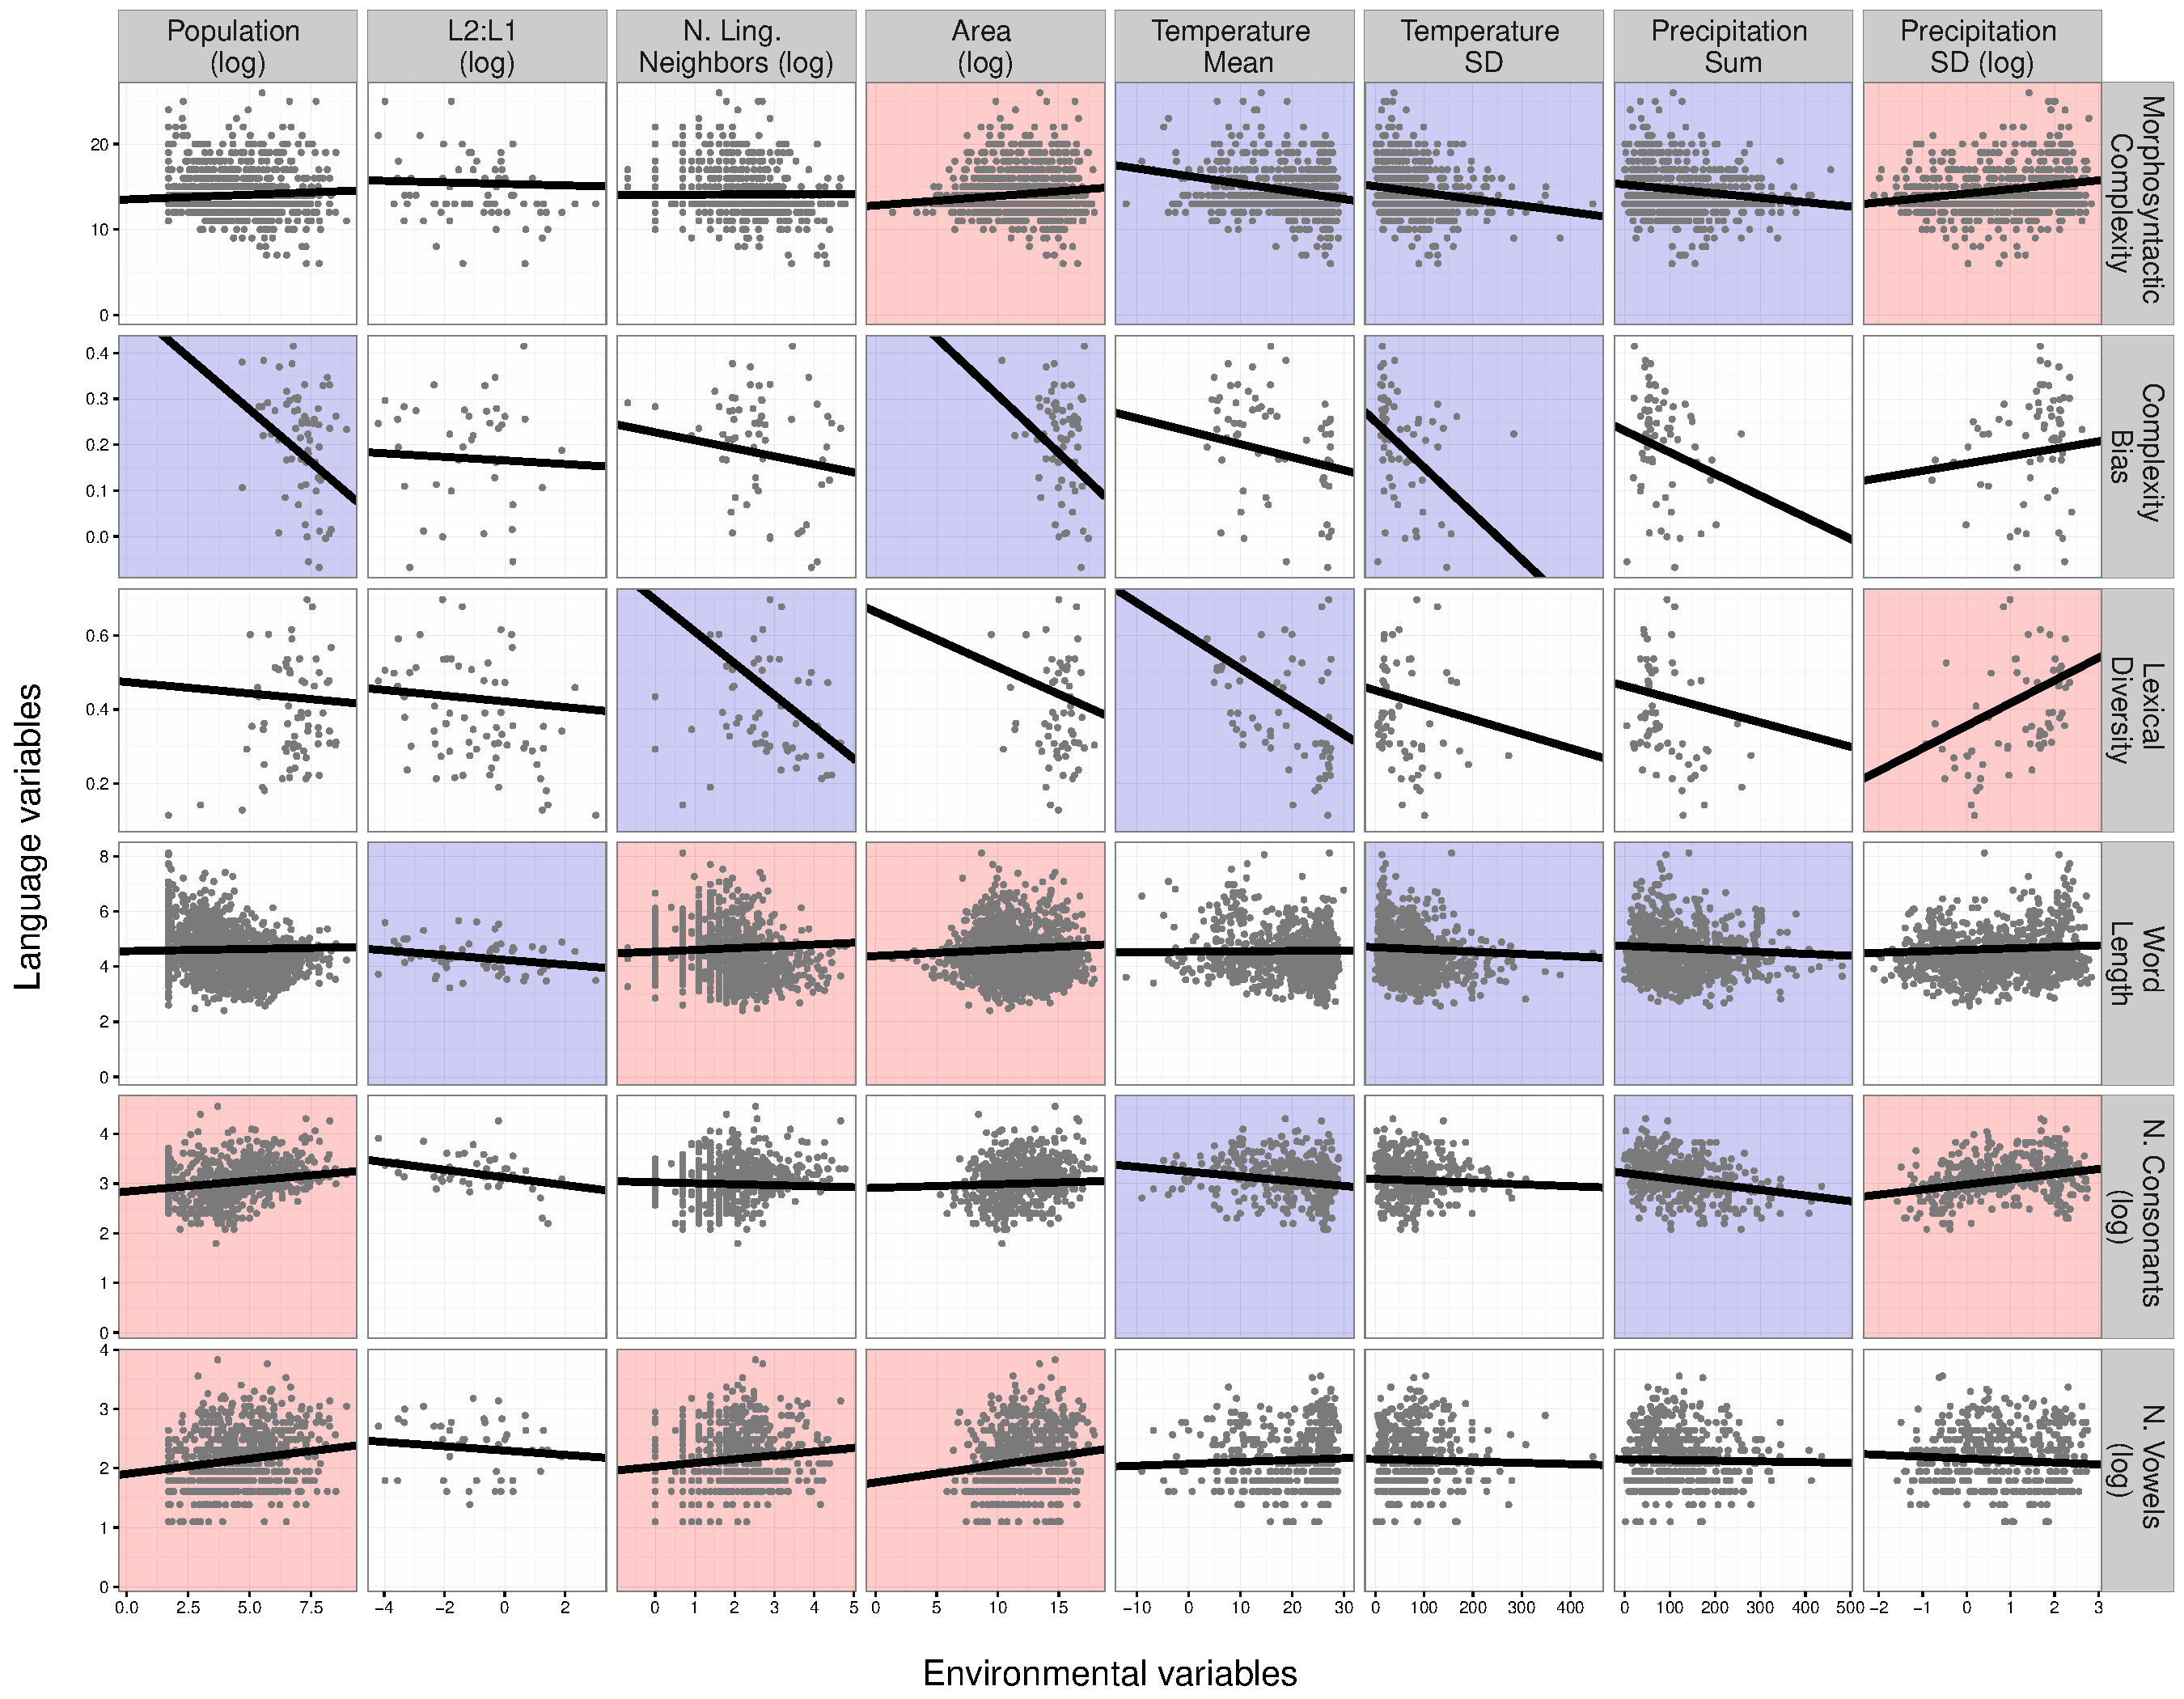
\includegraphics[scale = .38]{figs/plot1.pdf}
\end{center}
\vspace{-.5em}
\caption{Relationship between environmental and linguistic variables, which each point represents a language. Red (positive) and blue (negative) indicate models where the environmental variable is a significant predictor of the linguistic variable. Lines show the fixed effect estimate (slope) and  intercept of the mixed effect model. Number of languages varies across plots due to variation in the number of overlapping languages across datasets.}
\label{fig:cbias}
\vspace{-1em}
\end{figure*}

In this work, we try to address some of these challenges by clarifying the empirical landscape. We do this by aggregating across datasets that find covariation between environmental variables and linguistic structure. This serves two purposes. First, it allows us to examine the relationship between the same set of environmental predictors across a range of linguistic features. And, second, it allows for the same analytical techniques and areal controls to be used across datasets. By addressing these inconsistencies, we are better able to  directly compare relationships between environmental and linguistic features. A more coherent picture of the empirical landscape may in turn provide insight into the mechanism linking language systems to their environments.

We also directly explore the link between the acquisition and language evolution timescales by testing a novel prediction about the relationship between L1 and L2 learnability. If  the correlation between environments and linguistics complexity are due to different learning constraints of L1 and L2 learners, then we should expect different kinds of languages to favor acuisition for different populations. In particular, we explore the prediction that languages that are more easily learnable by L2 populations are harder to learn for L1 learners.

%We also more directly address the question of mechanism by examining variability in the mean age of acquisition of words for L1 learners across languages. Evidence that this variability is related to an aspect of the linguistic system (such as number of phonemes) would suggest that L1 learners, and not L2 learners, are the relevant environmental factor shaping that aspect of the linguistic system. 

In what follows, we first present a study examining the relationship between environmental and linguistic features using the same analytical techniques (Study 1). In Study 2, we examine the relationship between cross-linguistic variability in mean age of acquisition aspects of the environment and linguistic complexity.

%%%% Demo and language features%%%%%%
\section{Study 1: Environmental pressures on language systems}
The hypothesis of interest suggests a relationship between environmental and linguistic features, though the direction  and magnitude of this relationship varies across the previous literature. To explore this variation, we combined data from five existing datasets that included environmental or linguistic data. The datasets were selected for being publicly available and containing a large sample of languages. Below we describe each of these datasets, followed by our analytical method, and results.

\begin{figure*}[t]
\begin{center}
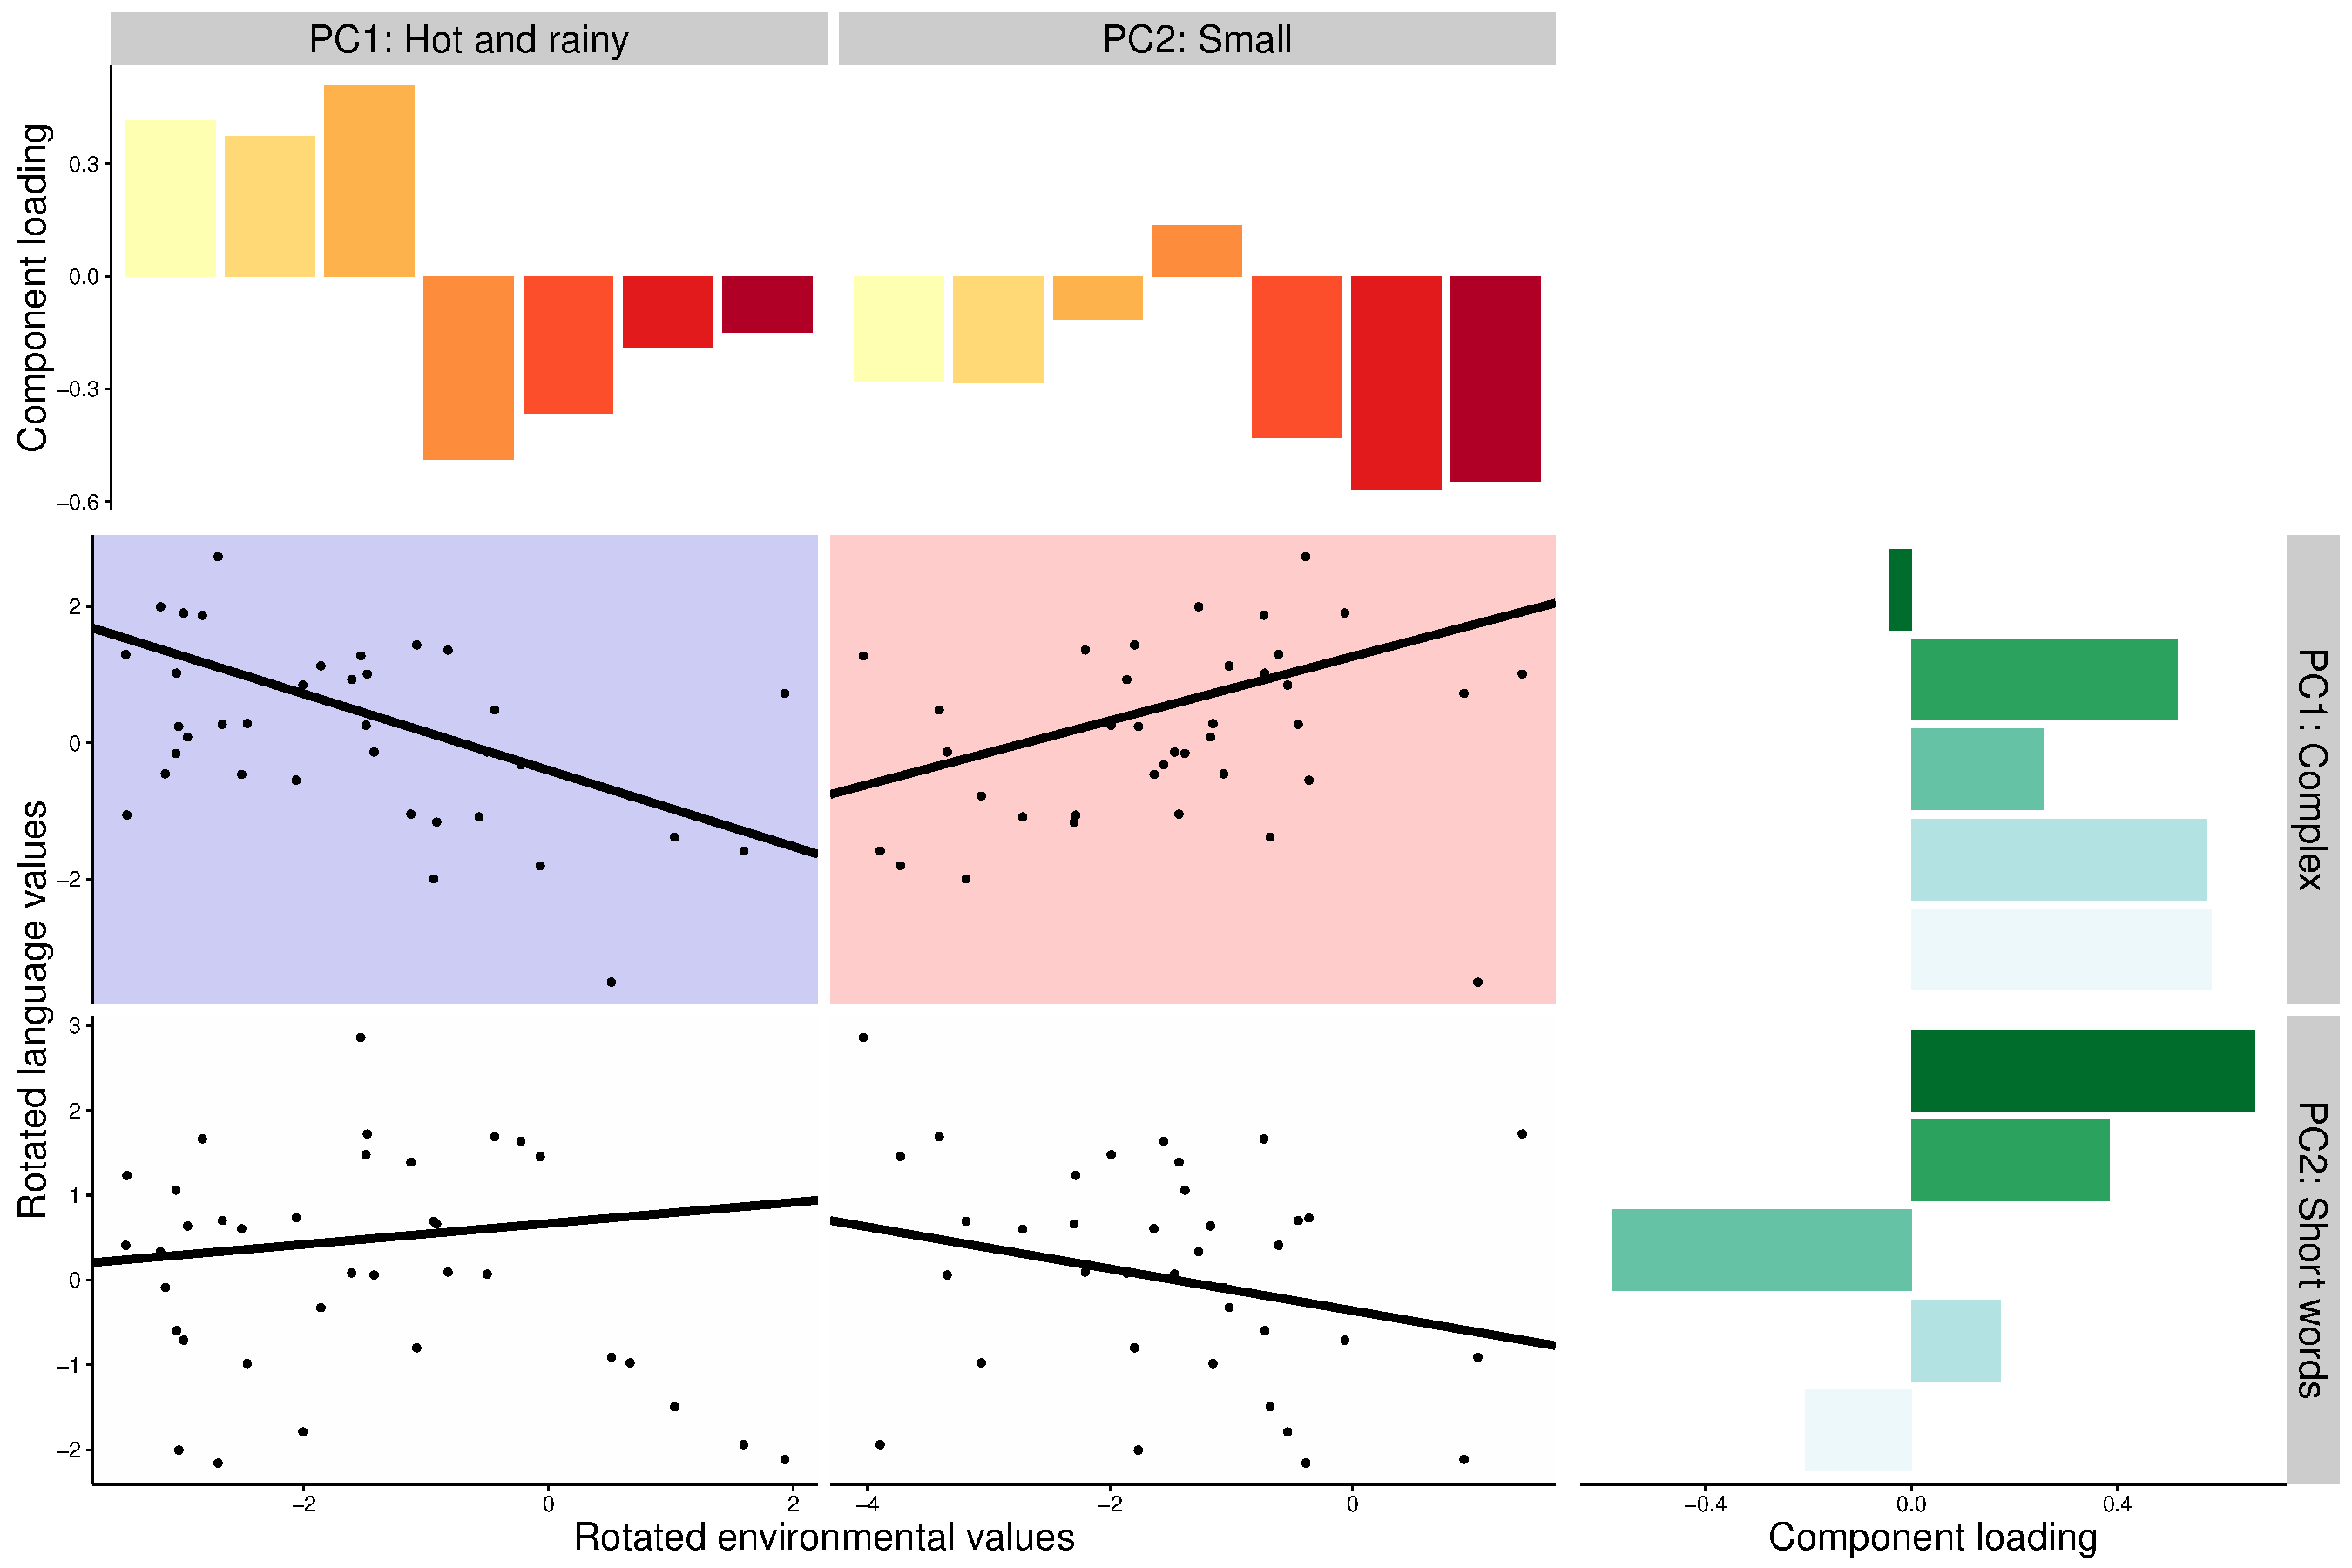
\includegraphics[scale = .35]{figs/plot2.pdf}

\end{center}
\vspace{-.5em}
\caption{Languages spoken in cold, small regions tend to be more complex. The bar plots show the loadings on the first two principal components for the environmental variables ($n$ = 7; orange) and language variables ($n$ = 5; green). The scatter plots show the relationship between the first two principal components for both sets of variables. Each point corresponds to a language, and lines show the linear fit from the mixed effect model. Significance and direction of a linear relationship are indicated by the coloring on the scatterplot (blue: significant and negative; red: significant  and positive).}
\label{fig:cbias}
\vspace{-1em}
\end{figure*}

\subsection{Datasets}
{\it Lupyan and Dale (2010).} This dataset contains grammatical information from WALS \cite{wals}, and demographic and geographic information from Ethnologue and the Global Mapping Institute \cite{gordon2005}. The demographic and geographic variables included total population of speakers, number of neighboring languages, area of region in which the language is spoken ($km$\textsuperscript{2}), mean and standard deviation temperature ($celsius$), and mean and standard deviation precipitation ($cm$). The metric of morphosyntactic complexity was calculated from  27 of the 28 morphosyntactic variables\footnote{WALS variable 59 was missing from the dataset.} analyzed in the original paper. For each variable, we coded the strategy as simple if it relied on a lexical strategy or few grammatical distinctions (e.g.,  0-3 noun cases), and complex if it relied on a morphological strategy or many grammatical distinctions (e.g.,  more than 3 noun cases). We summed the number of complex strategies to derive a measure of morphosyntactic complexity measure for each language, including only languages with data for all 27 variables. [$n$ = 1991] 
\cite{gmi}
{\it Bentz et al.\ (2015).} Two variables were used from this dataset: ratio of L2 to L1 speakers and number of word forms. Estimates of number of word forms were taken from translations of  {\it Universal Declaration of Human Rights}. Number of word forms was calculated as the number of unique words divided by the number of total words (type-token ratio). Higher type-token ratio indicates more word types in that language. Speaker population data were taken from a variety of sources, where L2 speakers were restricted to adult non-native speakers only. [$n$ = 81]

{\it Moran, McCloy and Wright (2012).} Estimates of number of consonants and vowels in each language were used from this dataset. These were originally taken from the Phoible database \cite{phoible}. [$n$ = 969]

{\it Lewis and Frank (2014).} This work finds that languages tend to map more complex meanings (measured via semantic norms) to longer words. The bias is estimated as the correlation (Pearson's $r$) between word length (in terms of number of characters) and complexity ratings for a set of 499 words translated via Google Translate. We used estimates of the correlation that partialed out the effect of spoken frequency [$n$ = 79]

{\it Wichmann, Rama, and Holman (2014).} This database contains translations for 40-lexical items across many languages. Word length was calculated as the mean number of characters in the ASJPcode transcription system across words in each language. [$n$ = 4421]

Aggregating across datasets, we analyzed 8 environmental variables in total: L2-L1 population ratio, total population size, number of neighbors, area of spoken region, mean and standard deviation temperature, and mean and standard deviation precipitation. These variables were selected from a larger set because they were not highly correlated with each other ($r<.8$). We analyzed 6 total linguistic variables: number of vowels, number of consonants, word length, type-token ratio, complexity bias, and morphosyntactic complexity.


\subsection{Method}
Datasets were merged using common ISO-639 codes. Five variables were log-transformed to better approximate a normal distribution (population, L2 to L1 ratio,  number of neighbors, area, number of consonants, number of vowels). 

We  tested for a linear relationship between each environmental and language variable.\footnote{All code and data for the paper are available at \url{http://github.com/mllewis/langLearnVar}}  A significant challenge in making inferences about language data is non-independence. This non-independence can come from at least two sources: genetic relatedness and language contact. Following \citeA{jaeger2011mixed}, we control for these factors statistically by using linear mixed-effects regression. We control for genetic non-independence by including a random intercept and slope by language family. We control for language contact by including country of origin as a random intercept (models with random slopes failed to converge).\footnote{The model specification was as follows:  \texttt{language.variable $\sim$ environmental.variable + (environmental.variable~\textbar~language.family) +  (1~\textbar~origin.country)}.}  We selected country of origin as a proxy for linguistic community because it was available for all languages in our dataset. Both control variables were taken from the WALS dataset. We considered a predictor significant if the test statistic on the fixed effect coefficient exceeded 1.96. 

\subsection{Results}
We fit mixed effect models predicting each language variable with each environmental variable using areal controls. The results are presented in Fig.\ 2. For each language variable, there was at least one environmental variable that reliably covaried. All significant effects are consistent with previous literature. Data can be explored interactively through an online app: [HERE].

This first analysis provides a uniform analysis of the many environmental and linguistic variables that have been used to test the Linguistic Niche Hypothesis. However,  the number of variables analyzed makes it difficult to distill a coherent picture from these data. Given that many of these variables  are partially correlated with each other, we used a technique for reducing the dimensionality of the dataset---principal component analysis. We found the principal components associated with the variance for the environmental variables and the linguistic variables, and then examined the relationship between the primary principal components. Complexity bias was excluded from this analysis since it was only available for a small subset of languages.

All variables were first scaled. For the environmental variables, the first two principal components accounted for  .69 of the total variance (PC1: .39; PC2: .30).  The weights on these variables across the two components can be seen in the upper panel of Fig.\ 3. The first component  loads most heavily on variables related to the climate. It can be thought of as corresponding to hot and rainy regions. The second component loads most heavily on variables related to the size of the region a language is spoken in, both in terms of number of speakers and physical size. This principal component can be roughly interpreted as the `smallness' of a linguistic community.

For the linguistic variables, the first two components also accounted for most of the variance, .70 (PC1: .39; PC2: .31; right panel of Fig.\ 3). The first component loads positively on all variables, except number of vowels. In particular, this component is associated with more consonants, longer words, more word types, and greater morphosyntactic complexity. Broadly, this component is related to the amount of cognitive difficulty associated with learning a language. The second component is associated with having short words, but large phonemic inventories. 

We then fit the same model as in the previous analysis using the rotated values for the first two principal components for the environmental and linguistic variables. Figure 3 shows the relationship between the principal components. Both environmental principal components were reliable predictors of the first linguistic principal component (PC1: $\beta=-0.56$; PC2: $\beta=0.47$). This suggests that languages that tend to be  spoken in cold and small regions are more likely to be more complex. Neither of the environmental principal components were reliable predictors of the second linguistic principal component.

\subsection{Discussion}
These two analyses suggest that more complex languages are spoken in cold, small regions. Importantly, we find this relationship across a range of linguistic features---morphosyntactic complexity, linguistic diversity, word length, and consonant inventory---using the same analytic technique across all measures. This finding is consistent with previous work that finds relationships between  individual metrics of complexity and various measures of population size \cite<e.g.,>{lupyan2010language}.

Why might there be this relationship? One mechanism consistent with these data is that languages spoken in larger places have more L2 learners, and that L2 learners are less skilled than L1 learners at acquiring complex languages. As a result, these languages adapt by simplifying. The relationship between climate and linguistic complexity is less clear, but one possibility is that speakers in  colder regions are less itinerant, and therefore have less contact with adult speakers of other languages.

%%%% AOA %%%%%%
\section{Study 2: Variability in L1 learning}
The proposed mechanism in Study 1 makes an important assumption: L2 learners, but not L1 learners, are poor learners of linguistic complexity.  \citeA{lupyanrole} have argued that morphological complexity in fact {\it facilitates} learning for L1 learners by providing redundancy in the linguistic signal. A straightforward prediction of this hypothesis is that languages that are more easily learnable by L2 learners will be less learnable by L1 learners. 

In Study 2, we explore this prediction. As a proxy for learnability for L1 learners, we use the mean age of acquisition (AoA) of words in a language. We predict that languages that  are more easily learnable by L1 speakers should have earlier AoAs that languages with a large L2 pressure.

\subsection{Method}
We use subjective measures of AoA from the the \citeA{luniewska2015ratings} norms. These AoAs were collected from adult participants for the translation equivalents of 299 words in 25 languages. To evaluate the validity of this measure, we compared these ratings to somewhat more objective measures of AoA collected from parent-report using the CDI \cite<Wordbank;>{frankwb}.  We fit a model predicting the objective ratings with the subjective ratings for the small sample of common languages ($n=7$). We included language as a random by-intercept and slope effect. Subjective ratings were a strong predictor of objective ratings ($\beta=1.00$, $t=5.45$), suggesting that the  \citeA{luniewska2015ratings} norms were a reasonable proxy for cross-linguistic AoA.
% or just correlaiotn: .36

We averaged across words in the \citeA{luniewska2015ratings} database to get a mean AoA for each language. We then used the same mixed-effect model as in Study 1 to predict AoAs with each of the linguistic and environmental variables analyzed in Study 1. 

\subsection{Results}
Across all models, three variables were reliable predictors of AoA: Number of consonants, variability in precipitation, and number of consonants. Temperature and number of consonants  was positively correlated with AoA  ($\beta=.13$, $t=2.57$;  $\beta=1.04$, $t=1.97$), and variability in precipitation was negative correlated ($\beta=-1.6$, $t=-2.83$).

\subsection{Discussion}
These results provide  preliminary support for the proposed tradeoff in learnability between L1 and L2 learners. Assuming that temperature and variability in precipitation are proxies for L2 pressure, we find that languages that have more L2 pressure have later AoAs, and therefore may be harder for L1 learners to acquire. The relationship between number of consonants and AoA is less straightforward to account for [WHAT TO SAY HERE].

\section{Conclusion}
Languages vary in many ways across multiple timescales of analysis. Here we suggest that this variability can be accounted for by considering the relationship between these timescales and two types of pressures, those internal and external to the cognitive system. In the present work, we have explored one hypothesis for variability at the language evolution timescale---the Linguistic Niche Hypothesis--- which suggests that cross-linguistic variability is the result of different cognitive constraints of learners and different environmental pressures.

We contribute to the empirical findings related to this hypothesis by synthesizing previous correlational evidence using common analytical techniques across datasets, and by testing a critical novel prediction of this hypothesis at the language acquisition timescale. Across a range of linguistic and environmental metrics,  we find that more complex languages tend to be spoken in smaller, colder regions. We also find evidence for a trade-off between  learnability for L1 and L2 speakers, consistent with one proposed mechanism for the relationship between languages and their environments.

Accounting for variability at the timescale of language evolution is an empirically challenging enterprise. We suggest that a fruitful avenue for progress is careful and complete descriptions of the empirical landscape, and appeals to processes at multiple timescales of analysis.


%Dale and luypan -- more stringent controls (monte carlo sampling in 2010 paper)

%Informative about the origins of language (~devo)
%Other attempts to get at this quesiton (modeling + experimental)
%Why? Cold and complex
%using Monte Carlo analyses to deal with Galton�s problem of non-independent sampling; Lupyan & Dale, 2010

%L2 vs. L1 learners might be good at different things

%QUESTIONS FOR MIKE:
%- maturation citaiton
%- how deal with lupyan different
%- cut citations?
%- secondarry dataset citations?
%- number of consonants and AoA - HELP
% working on shiny

%\cite{silvey2015word}
%\cite{perfors2011language}




%\cite{wichmann2011phonological}
%\cite{wichmann2008languagephonological}
%\cite{smith2010eliminating}
%\cite{slobin1982children}

%\cite{sapir1912language}
%\cite{reali2014paradox}


%\cite{lupyan2010language}
%This proposal is relatively uncontroversial at the level of semantics \cite{sapir}: Languages have words for meanings that are relevant for their environment (e.g. ). But, at  more abstract levels of language structure, this hypothesis has been very controversial. 
%\cite{kirby2008cumulative}
%Meaning. \cite{silvey2015word}
%\cite{perfors2011language}
%Critically, 



%\squeezeup


\section{Acknowledgments}
We would like to thank Gary Lupyan and Rick Dale for sharing their data with us.


\bibliographystyle{apacite}

\setlength{\bibleftmargin}{.125in}
\setlength{\bibindent}{-\bibleftmargin}

\bibliography{biblibrary}
\end{document}
